\documentclass[12pt, a4paper]{article}
\usepackage{amsmath}
\usepackage{graphicx}
\usepackage{listings}

\begin{document}

\section*{Ejemplos Numéricos. Reproducción de los experimentos}

Para reproducir los experimentos se utilizó el método de Runge-Kutta de orden 4 (RK4), programado
en Python 3.10 y haciendo uso de librerías para la manipulación eficiente de vectores como Numpy y 
Scipy.

El metodo de Runge-Kutta es método de un paso en el cual se usa un tamaño de paso $h$ para calcular 
los siguientes valores a partir de valores previos.

Como en este trabajo se utiliza un sistema de tres ecuaciones, 
es necesario de manera análoga crear otras variables $l$ y $m$ para
las funciones $y$ y $z$. El pseudocódigo sería de la siguiente manera:

\lstinputlisting[tabsize=2]{pseudocode.txt}

El tamaño de paso se estableció para todos los experimentos en 
$h=2^{-10}$ con el cual se obtienen resultados muy exactos teniendo
en cuenta que el error de RK4 es del orden $O(h^5)$, con lo que tendriamos
que el error sería aproximadamente del orden de $e \approx 2^{-50}$.

\subsection*{Reproducción de los experimentos}

Para los experimentos se utilizaron para los parámetros los valores de la siguiente tabla:

\begin{tabular}{p{1cm} | p{1cm} | p{1cm} | p{1cm} | p{1cm} | p{1cm} | p{1cm} | p{1cm} | p{1cm} }
    % aslask & gahbh
    $\#$ & $r$ & $\alpha$ & $\alpha_1$ & $\eta$ & $\eta_1$ & $K$ & $\rho$ & $m$\\
    1 & 0.82 & 1.56 & 1.12 & 2.41 & 1.83 & 12.0 & 1.38 & 0.13\\
    2 & 1.32 & 1.56 & 0.72 & 2.41 & 0.41 & 2.8 & 1.38 & 0.23\\
    3 & 1.32 & 0.76 & 0.72 & 0.6 & 0.41 & 2.8 & 0.78 & 0.23\\
    4 & 0.82 & 0.76 & 0.72 & 1.2 & 0.41 & 2.8 & 1.38 & 0.23\\
    5 & 1.32 & 1.16 & 0.72 & 0.31 & 0.41 & 2.8 & 0.78 & 0.23\\
\end{tabular}
\\
Además, se usó fijo $\beta=0.87$ y $\mu=0.11$.

\subsubsection*{Primer experimento}

En el primer conjunto de experimentos se usaron los valores iniciales $[x_0=3.01, y_0=5.05, z_0=4.28]$ (1.1)
y $[x_0=4.6, y_0=5.9, z_0=3.1]$(1.2). Como indica esta simulación, todas las poblaciones
pueden sobrevivir.

\begin{figure}[h!]
    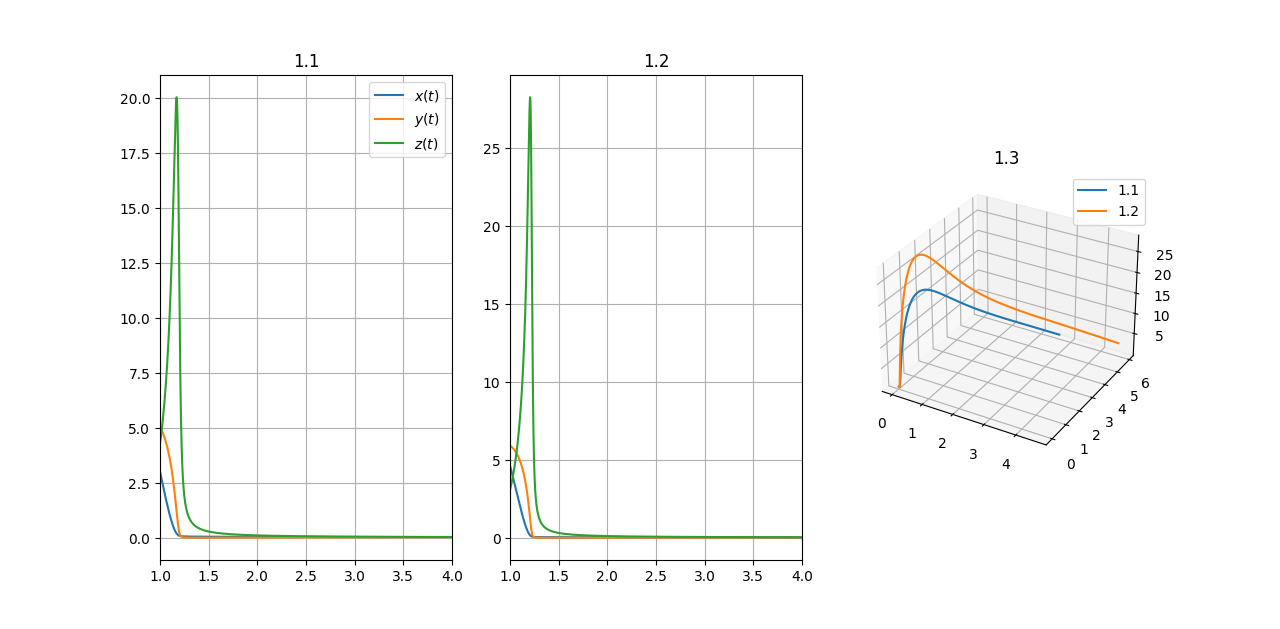
\includegraphics[width=\linewidth]{../images/1.png}
    \caption{Experimento \#1}
\end{figure}

\subsubsection*{Segundo experimento}

En el segundo conjunto de experimentos, se usaron valores tal que $\eta > \beta$ y $\eta > \alpha$. 
De valores iniciales se utilizaron $[x_0=0.3, y_0=2.4, z_0=3.9]$(2.1),
$[x_0=0.6, y_0=2.4, z_0=3.9]$(2.2) y $[x_0=2.1, y_0=1.2, z_0=1.1]$

La simulación muestra que todos los valores van al punto de equilibrio interior.

\begin{figure}[h!]
    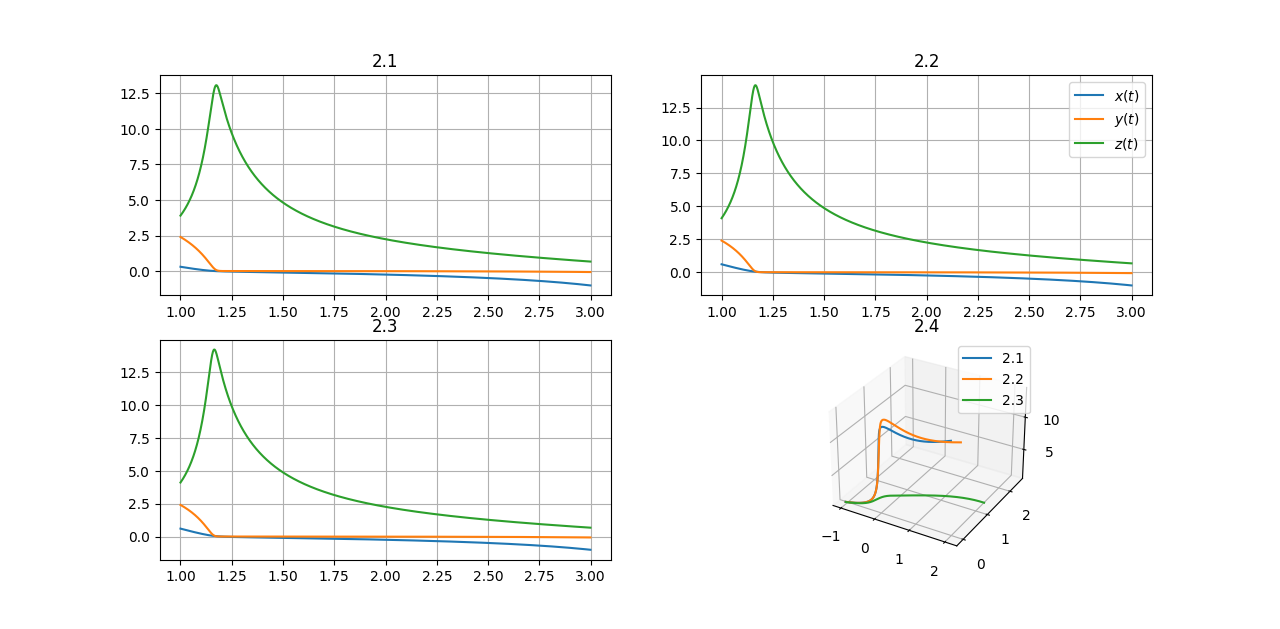
\includegraphics[width=\linewidth]{../images/2.png}
    \caption{Experimento \#2}
\end{figure}

\subsubsection*{Tercer experimento}

En el tercer experimento, se usaron valores tal que $\alpha > \beta$
Los valores iniciales usados fueron $[x_0=0.3, y_0=2.4, z_0=3.9]$. La simulación muestra 
que los valores van al punto de equilibrio.

\begin{figure}[h!]
    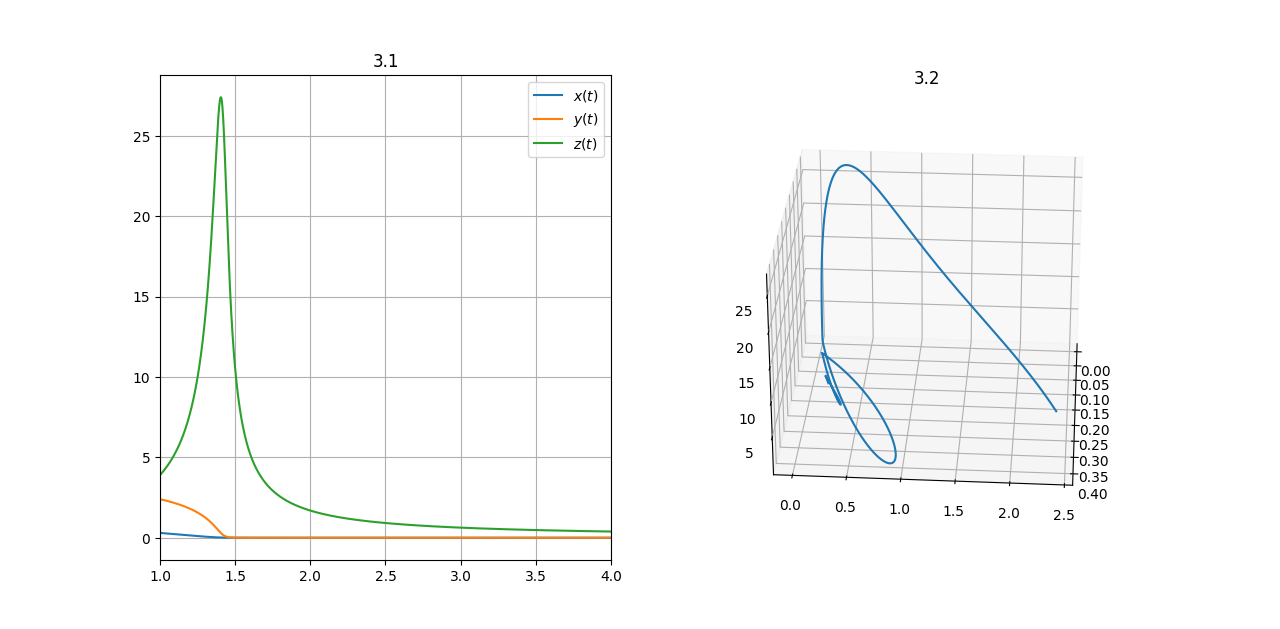
\includegraphics[width=\linewidth]{../images/3.png}
    \caption{Experimento \#3}
\end{figure}

\subsubsection*{Cuarto experimento}

En el cuarto experimento, se usaron valores tal que $\eta = \alpha$.
Los valores iniciales usados fueron $[x_0=1.2, y_0=2.1, z_0=4.28]$. La simulación muestra 
que los valores van al punto de equilibrio.

\begin{figure}[h!]
    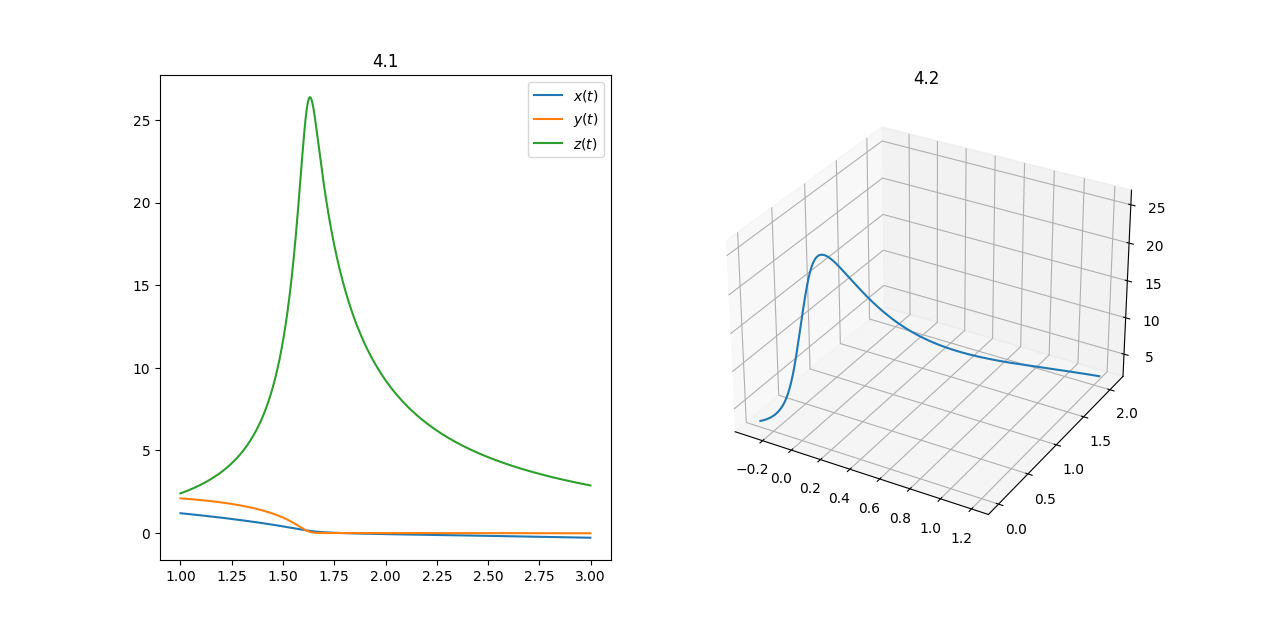
\includegraphics[width=\linewidth]{../images/4.png}
    \caption{Experimento \#4}
\end{figure}

\subsubsection*{Quinto experimento}

En el quinto experimento, se usaron valores tal que $\eta > \beta$ y $\eta > \alpha$.
Los valores iniciales usados fueron $[x_0=1.2, y_0=2.1, z_0=2.4]$. La simulación muestra 
que los valores van al punto de equilibrio.

\begin{figure}[!h]
    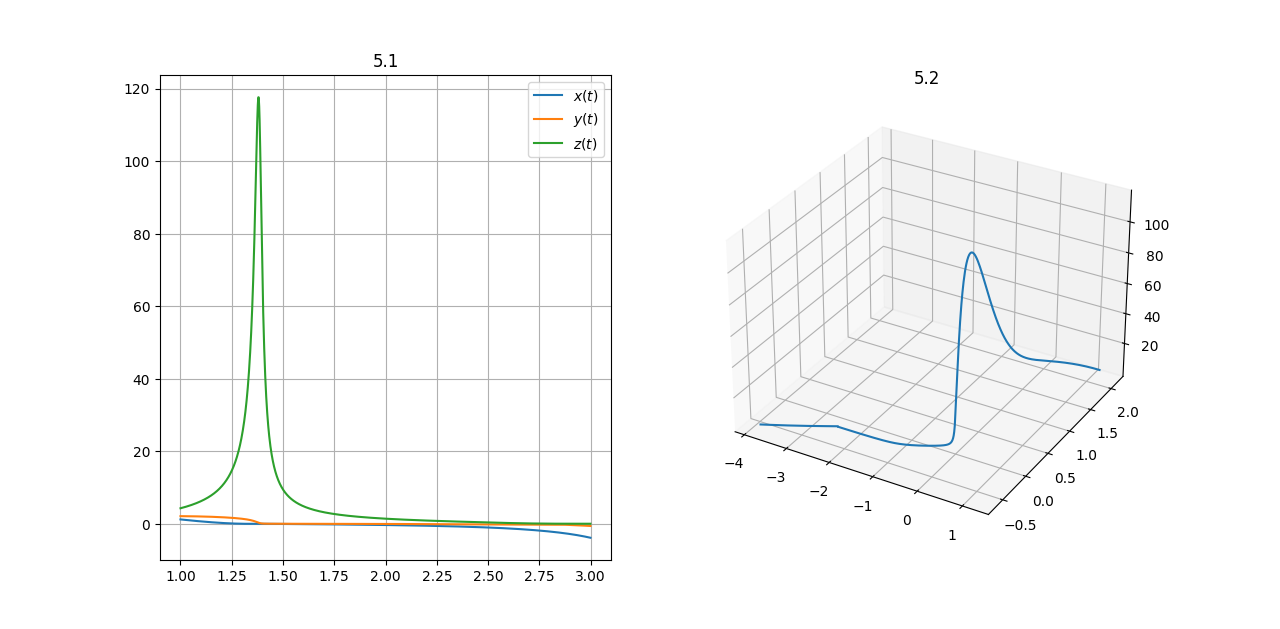
\includegraphics[width=\linewidth]{../images/5.png}
    \caption{Experimento \#5}
\end{figure}

\end{document}